\documentclass[14pt]{extbook}
\usepackage{multicol, enumerate, enumitem, hyperref, color, soul, setspace, parskip, fancyhdr} %General Packages
\usepackage{amssymb, amsthm, amsmath, latexsym, units, mathtools} %Math Packages
\everymath{\displaystyle} %All math in Display Style
% Packages with additional options
\usepackage[headsep=0.5cm,headheight=12pt, left=1 in,right= 1 in,top= 1 in,bottom= 1 in]{geometry}
\usepackage[usenames,dvipsnames]{xcolor}
\usepackage{dashrule}  % Package to use the command below to create lines between items
\newcommand{\litem}[1]{\item#1\hspace*{-1cm}\rule{\textwidth}{0.4pt}}
\pagestyle{fancy}
\lhead{Progress Quiz 6}
\chead{}
\rhead{Version A}
\lfoot{4563-7456}
\cfoot{}
\rfoot{Summer C 2021}
\begin{document}

\begin{enumerate}
\litem{
For the scenario below, use the model for the volume of a cylinder as $V = \pi r^2 h$.
\begin{center}
    \textit{ Pringles wants to add 42 \text{percent} more chips to their cylinder cans and minimize the design change of their cans. They've decided that the best way to minimize the design change is to increase the radius and height by the same percentage. What should this increase be? }
\end{center}
\begin{enumerate}[label=\Alph*.]
\item \( \text{About } 21 \text{ percent} \)
\item \( \text{About } 3 \text{ percent} \)
\item \( \text{About } 12 \text{ percent} \)
\item \( \text{About } 19 \text{ percent} \)
\item \( \text{None of the above} \)

\end{enumerate} }
\litem{
For the scenario below, use the model for the volume of a cylinder as $V = \pi r^2 h$.
\begin{center}
    \textit{ Pringles wants to add 33 \text{percent} more chips to their cylinder cans and minimize the design change of their cans. They've decided that the best way to minimize the design change is to increase the radius and height by the same percentage. What should this increase be? }
\end{center}
\begin{enumerate}[label=\Alph*.]
\item \( \text{About } 3 \text{ percent} \)
\item \( \text{About } 10 \text{ percent} \)
\item \( \text{About } 15 \text{ percent} \)
\item \( \text{About } 16 \text{ percent} \)
\item \( \text{None of the above} \)

\end{enumerate} }
\litem{
Solve the modeling problem below, if possible.
\begin{center}
    \textit{ A new virus is spreading throughout the world. There were initially 6 many cases reported, but the number of confirmed cases has doubled every 4 days. How long will it be until there are at least 10000 confirmed cases? }
\end{center}
\begin{enumerate}[label=\Alph*.]
\item \( \text{About } 43 \text{ days} \)
\item \( \text{About } 15 \text{ days} \)
\item \( \text{About } 30 \text{ days} \)
\item \( \text{About } 14 \text{ days} \)
\item \( \text{There is not enough information to solve the problem.} \)

\end{enumerate} }
\litem{
Determine the appropriate model for the graph of points below.
\begin{center}
    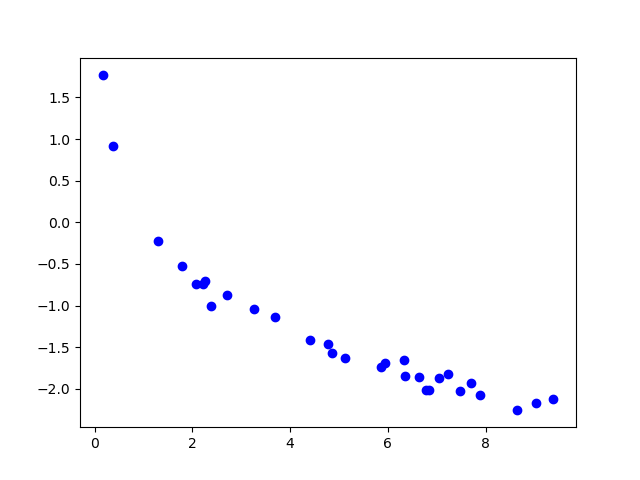
\includegraphics[width=0.5\textwidth]{../Figures/identifyModelGraph12CopyA.png}
\end{center}
\begin{enumerate}[label=\Alph*.]
\item \( \text{Logarithmic model} \)
\item \( \text{Exponential model} \)
\item \( \text{Non-linear Power model} \)
\item \( \text{Linear model} \)
\item \( \text{None of the above} \)

\end{enumerate} }
\litem{
Determine the appropriate model for the graph of points below.
\begin{center}
    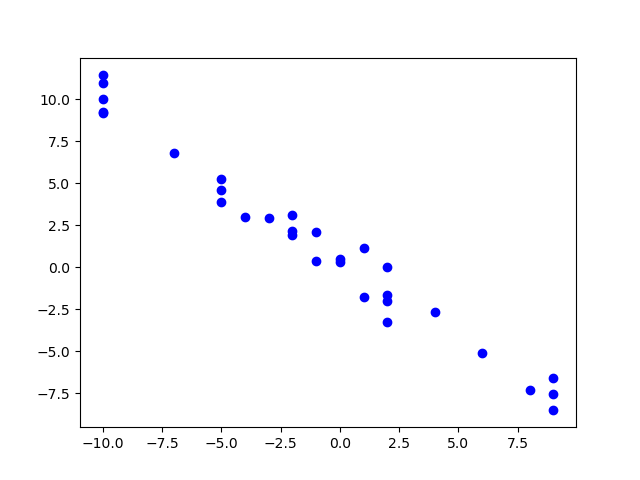
\includegraphics[width=0.5\textwidth]{../Figures/identifyModelGraph12A.png}
\end{center}
\begin{enumerate}[label=\Alph*.]
\item \( \text{Non-linear Power model} \)
\item \( \text{Linear model} \)
\item \( \text{Exponential model} \)
\item \( \text{Logarithmic model} \)
\item \( \text{None of the above} \)

\end{enumerate} }
\litem{
\begin{enumerate}[label=\Alph*.]

\end{enumerate} }
\litem{
Solve the modeling problem below, if possible.
\begin{center}
    \textit{ In CHM2045L, Brittany created a 18 liter 31 percent solution of chemical $\chi$ using two different solution percentages of chemical $\chi$. When she went to write her lab report, she realized she forgot to write the amount of each solution she used! If she remembers she used 15 percent and 37 percent solutions, what was the amount she used of the 37 percent solution? }
\end{center}
\begin{enumerate}[label=\Alph*.]
\item \( 9.00 liters \)
\item \( 7.93 liters \)
\item \( 4.91 liters \)
\item \( 13.09 liters \)
\item \( \text{There is not enough information to solve the problem.} \)

\end{enumerate} }
\litem{
Solve the modeling problem below, if possible.
\begin{center}
    \textit{ A new virus is spreading throughout the world. There were initially 5 many cases reported, but the number of confirmed cases has tripled every 4 days. How long will it be until there are at least 10000 confirmed cases? }
\end{center}
\begin{enumerate}[label=\Alph*.]
\item \( \text{About } 31 \text{ days} \)
\item \( \text{About } 15 \text{ days} \)
\item \( \text{About } 28 \text{ days} \)
\item \( \text{About } 14 \text{ days} \)
\item \( \text{There is not enough information to solve the problem.} \)

\end{enumerate} }
\litem{
Solve the modeling problem below, if possible.
\begin{center}
    \textit{ In CHM2045L, Brittany created a 16 liter 26 percent solution of chemical $\chi$ using two different solution percentages of chemical $\chi$. When she went to write her lab report, she realized she forgot to write the amount of each solution she used! If she remembers she used 20 percent and 38 percent solutions, what was the amount she used of the 38 percent solution? }
\end{center}
\begin{enumerate}[label=\Alph*.]
\item \( 10.67 liters \)
\item \( 8.00 liters \)
\item \( 5.26 liters \)
\item \( 5.33 liters \)
\item \( \text{There is not enough information to solve the problem.} \)

\end{enumerate} }
\litem{
For the information below, construct a linear model that describes the total time $T$ spent on the path in terms of the distance of a particular part of the path \textit{if we know that all parts of the path are equal length}.
\begin{center}
    \textit{ A bicyclist is training for a race on a hilly path. Their bike keeps track of their speed at any time, but not the distance traveled. Their speed traveling up a hill is 6 mph, 10 mph when traveling down a hill, and 8 mph when traveling along a flat portion. }
\end{center}
\begin{enumerate}[label=\Alph*.]
\item \( 24.000 D \)
\item \( 480.000 D \)
\item \( 0.392 D \)
\item \( \text{The model can be found with the information provided, but isn't options 1-3.} \)
\item \( \text{The model cannot be found with the information provided.} \)

\end{enumerate} }
\end{enumerate}

\end{document}